\documentclass{article}[20pt]
\usepackage{amsmath}
\usepackage{amsfonts}
\usepackage{graphicx}
\usepackage{enumerate}
\usepackage{dtklogos}
\usepackage{verbatim}
\usepackage{url}
\usepackage{natbib}
\usepackage{caption}

\usepackage{calrsfs}
\usepackage{collectbox}
\usepackage{blindtext}
\newcommand{\R}{{\mathbb R}}
\renewcommand{\vec}[1]{{\mathbf #1}}
\newcommand{\points}[1]{\phantom{.}\hfill \textbf{(#1 points)}}
\newcommand{\matlab}{{\textsc{Matlab}} }


\begin{document}
\begin{center}


\title{Seminar - Cook's Distance }
\hfill Iliass Tiendrebeogo\\

\hfill \today\\
\end{center}
\bigskip

\begin{center}
  \begin{Large}
      
    Seminar 4 - Cook's Distance \\
    Math 567: Winter 2016 \\
       
  \end{Large}
\end{center}

\bigskip

In Regression analysis, Cook's Distance is used to estimate the influence of a data point over the model when performing the ordinary least square regression method. It was introduced by R. Dennis Cook in 1977. \citep{cook} 
\section{Highly influential  data point}
A data point is said to be influential if when removed from the calculation change the regression line significantly. Data point with high leverage can be influential it is an outlier. However, a data point can have an high leverage but not influential, and it goes the same way for an outlier(all outlier are not influential).

The {\bf leverage} define how far apart is a given data point from the average(mean/median). Points with high leverage tend to pull the regression line toward themselves and have impact on the slop of the regression line hence {\bf influential}.
\section{Cook's Distance}
Cook's distance measures how much a parameter estimate change when a data-point is removed from the calculation. Data points with large residuals (outliers) and/or high leverage may distort the outcome and accuracy of a regression. Points with a large Cook's distance needs closer examination in the analysis.

\bigskip
The algebraic expression.
$$D_i = \frac{\sum_{j=1}^n \left( \hat{Y}_j - \hat{Y}_{j(i)}  \right) ^2}{k MSE}$$
Where:\\
$\hat{Y}_j$ is the prediction from the full regression model for observation $j$; \\
$\hat{Y}_{j(i)}$ is The prediction for observation $j$ from a refitted regression model in which observation $i$ has been omitted;\\
$k$ is the number of prediction parameter of the regression model;\\
$MSE$ is the mean square error.\\


\section{Interpretation of Cook's Distance}
There are several rules when interpreting {\bf cook's distance}. The widely used criterion is that a point is considered to be highly influential if $D_i > 1$ \citep{weisberg}

Different rules have  been defined such as: $D_i > 0.85$ if $p > 3$ \citep{barry}   where $p$ is the number of regression parameter. \citep{Robert} declares a data-point to be influential when $D_i > \frac{4}{n}$ where $n$ is the number of observation.
\section{Cook's Distance using R}
In this example we use album sales2 data from the book "Discovering Statistics Using R" \citep{DSUR}\\
First we build the fitted regression model after loading the data \\
\texttt{album2<-read.delim("Album Sales 2.dat", header = TRUE)\\
\# run the multiple regression model\\
lm\_model<-lm(sales ~ adverts + airplay + attract, data = album2)\\
\# analyse the cook's D by calling the built-in function cooks.distance\\
cooks.D <- cooks.distance(lm\_model)\\
\# determine influential points by applying the threshold of 0.05 \\
influential <- cooks.D > 0.05\\
we managed to isolate points at positions 1, 164, 169}\\
Now we plot cook's Distance vector\\
\texttt{plot(cooks.D, ylab = "cook's distance")\\
\# point with high $D_i$ will be shown red\\ 
points(1, cooks.D[1], col = 'red') \\
points(164, cooks.D[164], col = 'red')\\
points(169, cooks.D[169], col = 'red')}
\begin{figure}[]
\begin{center}
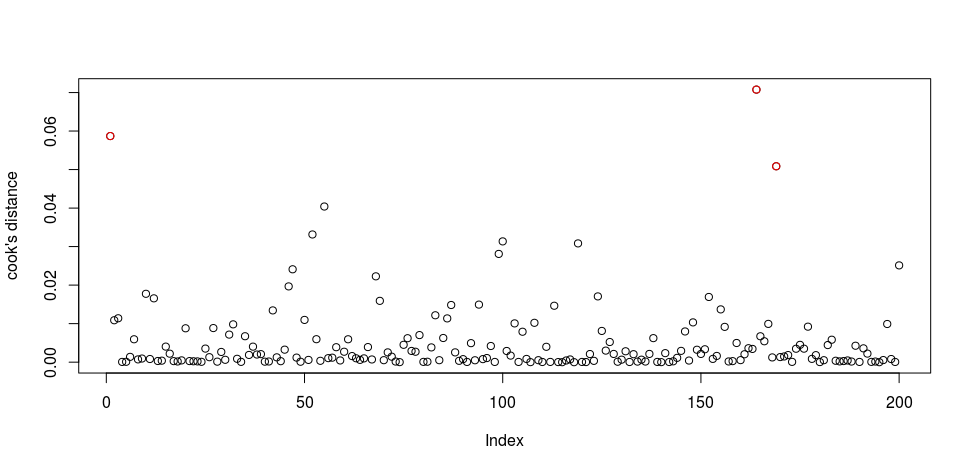
\includegraphics[width=\linewidth]{cooksd}
\end{center}
\caption{Cook's Distance on 200 album sales data}

\label{fig:figure1}
\end{figure}

\newpage

\section{Discussion}
{ \bf What should we do when a given data-point's $D_i > threshold$ ?:}\\


First we should make sure that the observation is recorded correctly.\\
Do the outcome change when the data is removed from the calculation? if the outcome do not change, it's not a big deal, but if the outcome change then this a problem that we need to fix. We don't want our statistical model relaying on a single data-point.\\

In that case we could reports two different results , one whit the influential data and another one without the the influential data.\\

Or we could restrict the analysis to values of $X$ for which the relationship holds. Which is usually not a good idea since we are omitting a data-point even though we would report that a outlier has been removed from the calculation. 



\bigskip


\bibliographystyle{plainnat}
\bibliography{cooks_distance}
\end{document}